\section{Introduction}
\label{sec:intro}
Time series forecasting underpins decision-making across diverse domains such as finance, energy, climate science, and healthcare, playing a pivotal role in tasks including weather forecasting~\citep{weathernature2025,wu2021autoformer}, energy consumption planning~\citep{lai2018energy,alvarez2010energy,cheng2021windturbine}, traffic scheduling~\citep{cirstea2022towardstraffic,cirstea2021enhancenet,wu2021autocts}.
\blue{Many of these series are spatio-temporal: they are produced by large networks of sensors, such as loop detectors on a road network or smart meters on a power grid, and a forecasting system must serve every sensor of the network continuously. In this setting the cost of a model is multiplied by the number of sensors and by the frequency of re-forecasting, so efficiency and scalability are first-class requirements alongside accuracy~\citep{lai2023lightcts}.}
In recent years, deep learning has demonstrated promising potential in this field by leveraging end-to-end modeling and powerful representational capacity to extrapolate from history to future trends.

A central inductive bias in forecasting models is periodicity--the recurring temporal structure inherent in many real-world time series.
Periodicity is ubiquitous in practice, appearing in domains ranging from urban traffic flow to cloud resource utilization and other workloads, making periodicity-aware modeling broadly applicable~\citep{deng2024disentangling, xia2025timeemb}.
Recent advances exploited this property by segmenting sequences into patch tokens, potentially aligned with cycles, prior to processing by the crafted models~\citep{nie2023patchtst, zhang2023crossformer, huang2025timebase, tang2025unlocking}.
For instance, \cite{nie2023patchtst} applied Transformer to tokenized time series to capture temporal correlations within and between cycles, while \cite{zhang2023crossformer} extended this paradigm by modeling cross-dimension dependencies and cross-scale interactions.

\begin{figure*}[t]
  \centering
  \begin{subfigure}[t]{0.49\textwidth}
    \centering
    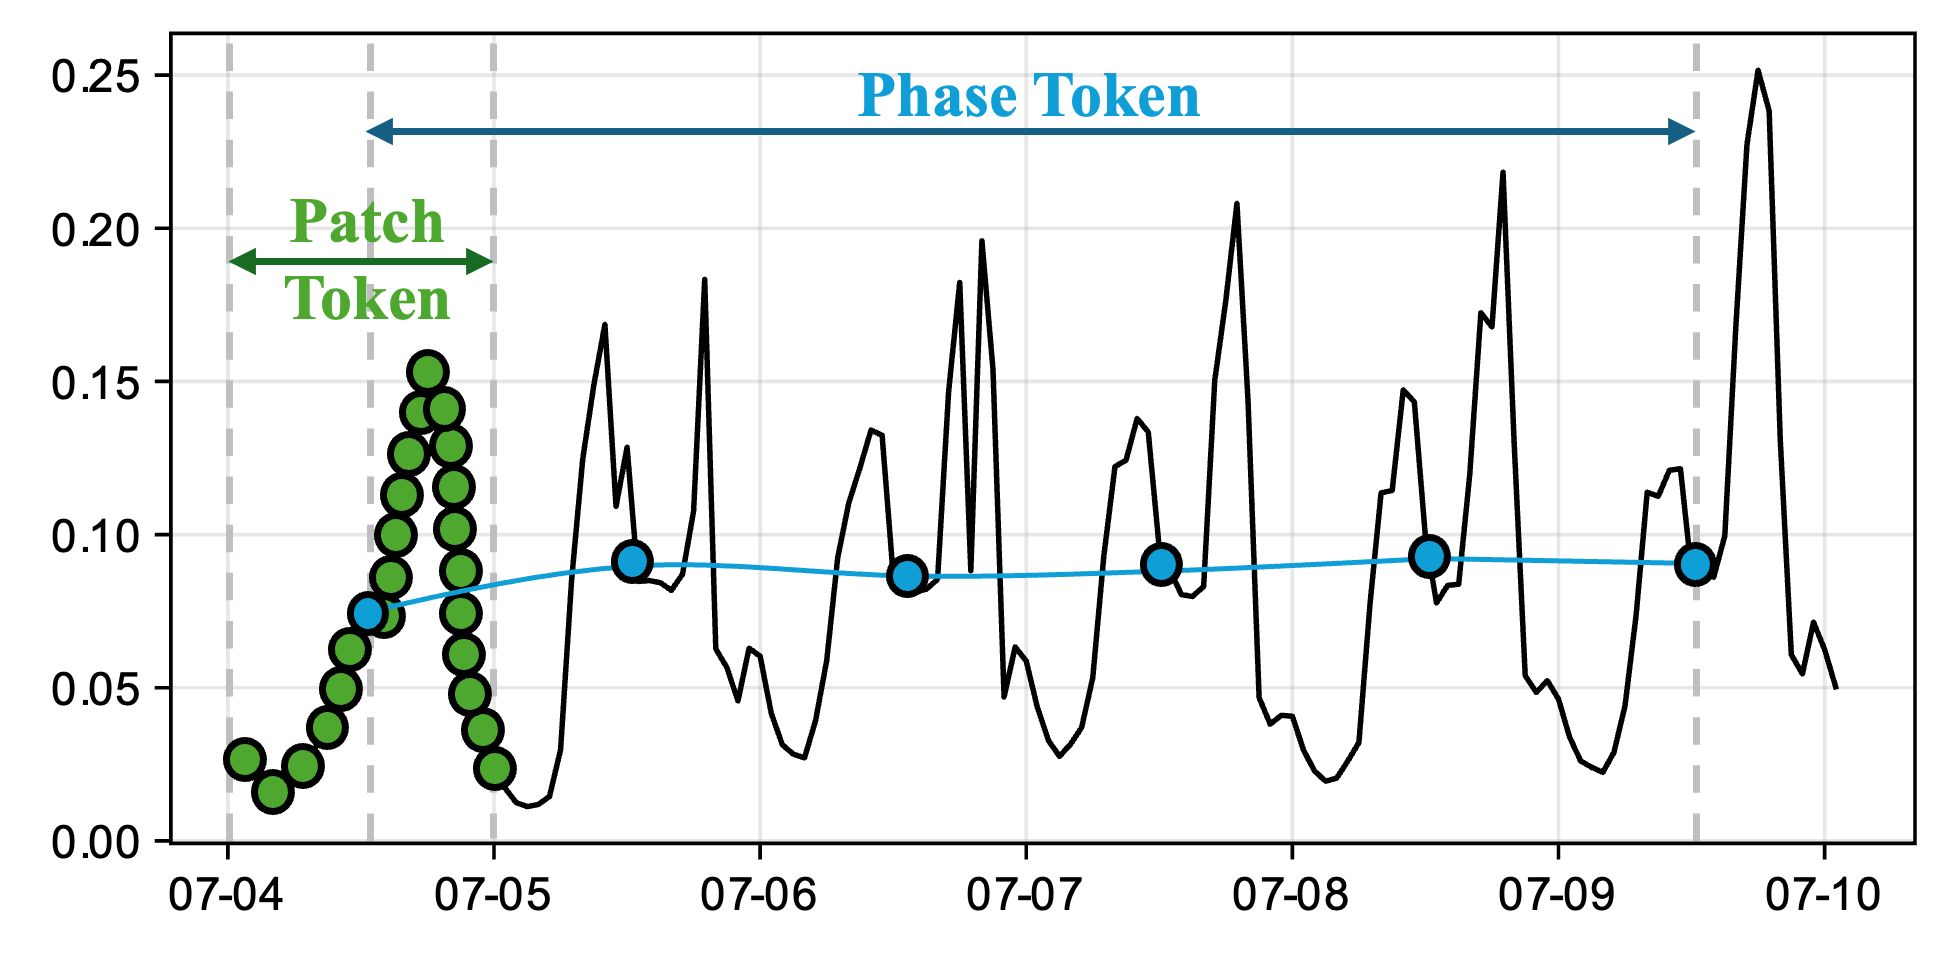
\includegraphics[width=\linewidth]{figures/phase_token.png}
    \caption{Patch Token vs. Phase Token.}
    \label{fig:phase_token}
  \end{subfigure}
  \hfill
  \begin{subfigure}[t]{0.49\textwidth}
    \centering
    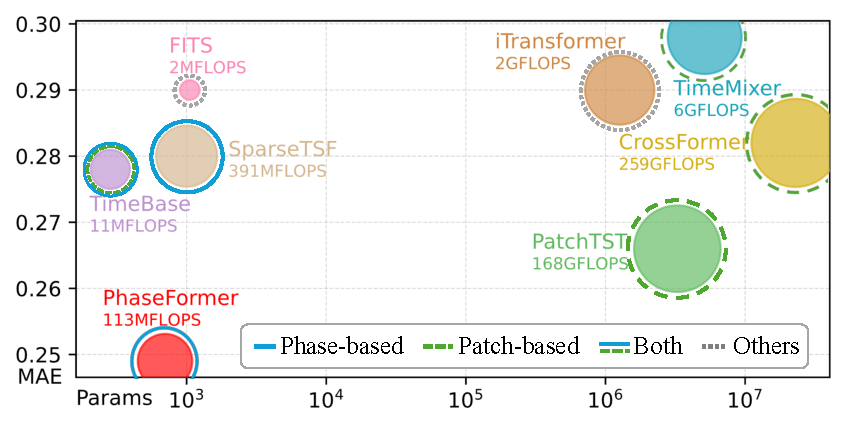
\includegraphics[width=\linewidth]{figures/efficiency_plot.pdf}
    \caption{Model Accuracy and Efficiency Comparison.}
    \label{fig:efficiency_plot}
  \end{subfigure}
  \caption{Comparison between patch-based and phase-based representations for time-series forecasting. (a) illustrates the difference in tokenization. (b) provides a joint evaluation of model accuracy, parameter scale, and computational overhead on the Traffic dataset, using an input length of 720 steps and predicting 96 future steps, where the marker size denotes the FLOPs.}
  \label{fig:introduction}
\end{figure*}

Despite their effectiveness, patch-based approaches struggle to scale efficiently to large and complex datasets~\citep{nie2023patchtst, zhang2023crossformer,tang2025unlocking}.
\emph{We attribute this poor scalability to the substantial variability of cycle patterns in real-world scenarios}.
This variability stems from dynamic external factors, which continuously shift the cycle patterns. For instance, traffic flow patterns may evolve as new infrastructure is introduced, while electricity demand can change with adjustments in work schedules~\citep{shao2025hutformer, shao2025hyperd, zhou2025feddis}.
This variability forces models to construct a high-dimensional representation space to faithfully accommodate the broadened distribution, which inevitably inflates both parameter counts and computational costs~\citep{shao2025blast}.
Additionally, these methods also struggle to generalize under such varying behavior, resulting in unreliable forecasts for samples beyond training data.

To address this challenge, we introduce a phase-based perspective that focuses on values aligned at the same offset across successive cycles. From this perspective, the dynamics of a time series are characterized by the cross-period trends of each phase--captured as phase tokens--while disregarding the full cyclic behavior. As illustrated in Fig.~\ref{fig:phase_token}, phase tokens exhibit significantly lower variability than patch tokens, enabling more efficient and generalizable representation, which in turn makes \sysname well suited for resource-constrained environments.
Importantly, excluding cycle patterns has minimal impact on forecasting effectiveness, since the cyclic behaviors remain locally stable and thus require little effort to predict. We study and verify these properties in depth in Sec.~\ref{sec:motivations} using real-world data, showing the stationarity and compactness of the feature space offered by phase tokenization.

Building on these insights, we propose Phase-based Routing Transformer, abbreviated as \textbf{\sysname}, which reframes time series as a collection of phase tokens and casts step-wise prediction as phase-wise prediction. Specifically, \sysname (i) aligns and extracts phase tokens from the input sequence and maps them into a shared low-dimensional latent space, (ii) employs a lightweight routing mechanism to enable efficient communication across phases, and (iii) applies a shared predictor to project the latent representations into forecasts for each phase. Extensive experiments demonstrate that, compared with PatchTST~\citep{nie2023patchtst} and Crossformer~\citep{zhang2023crossformer}, \sysname achieves over \textbf{99.9\%} reduction in both parameter count and computational cost, while delivering consistent improvements in prediction accuracy across all seven benchmark datasets, as illustrated by the Traffic dataset in Fig.~\ref{fig:efficiency_plot}.
Moreover, in contrast to methods with comparable efficiency such as SparseTSF~\citep{lin2024sparsetsf} and TimeBase~\citep{huang2025timebase}, \sysname significantly enhances predictive effectiveness, particularly on large and complex datasets.
Finally, we conduct a comprehensive analysis of different configurations to reveal the necessity of the constructed components and the effects of various hyperparameters.

\blue{
\fakeparagraph{Beyond stable cycles}
The conference version of this work~\citep{niu2026phaseformer} explained the efficiency of phase tokens with a stability theorem: when the recurring shape of a cycle is transformed in the same way in every cycle, the phase subspace does not move, whereas the patch subspace does. This covers changes \emph{along the phase axis} of the folded series. Real sensor streams also change \emph{along the cycle axis}: the level of a road segment's daily profile drifts from week to week, and the amplitude of that profile grows and shrinks with the level, as in the classical multiplicative seasonality of Holt--Winters~\citep{winters1960forecasting}. Such changes add new directions to the phase subspace, so they fall outside the conference theorem. The conference version left them as its main limitation: \sysname ``assumes locally stable periodicity'', and modeling ``non-stationarity and complex drifts'' was named as future work.

In this extended version, we close this gap theoretically and architecturally while keeping the efficiency that motivates phase tokens. We show that \sysname is not blind to cycle-axis changes: a level shift passes exactly through the routing layer, and the architecture can approximate the Bayes forecast of a seasonal random-walk model. Its capacity is, however, bounded by an \emph{envelope} that is fixed by the final layer normalization and can be read from the trained weights. We prove two such envelopes, one for the cycle level and one for a level-dependent amplitude, and show that what lies outside each envelope has a simple structure. The unmodeled level acts only through a few fixed horizon profiles, so a rank-3 linear branch on cycle means can carry it. The unmodeled amplitude is a bilinear product of level and shape, so a centered multiplicative modulation of the phase latent can carry it, and we prove that this modulation leaves every future cycle mean unchanged, so it does not disturb the level guarantees. The resulting model, \textbf{\sysLA}, keeps the conference architecture unchanged and adds at most a few hundred parameters, independent of the forecast horizon.
}

Our contributions are as follows:

\begin{enumerate}[leftmargin=2em]
\item We introduce a phase-based perspective that aligns values across cycles for the characterization of long-term time series, empirically and theoretically demonstrating improved feature stationarity and compactness over the patch-based perspective.

\item We propose \sysname, a lightweight forecasting model that reframes time series as phase tokens, maps them into a shared latent space, and employs a low-rank routing mechanism specifically designed around phase tokens to enable efficient phase-wise forecasting.

\item Extensive experiments are conducted to showcase that \sysname achieves substantial efficiency gains while consistently improving forecasting accuracy, establishing a superior efficiency–effectiveness trade-off across diverse benchmarks.

\blue{\item We characterize the limits of phase tokenization under cycle-axis changes. We prove a capability result and two envelope theorems, for the level and for the amplitude of cycles, and two complement theorems that identify the minimal structure needed beyond each envelope (Section~\ref{sec:theory}).}

\blue{\item We derive \sysLA from these results: a rank-3 level branch on cycle means with fixed horizon profiles, and a centered amplitude modulation that provably preserves every future cycle mean. Both add at most a few hundred parameters (Section~\ref{sec:extension}).}

\blue{\item We provide a data-centric analysis of level--amplitude coupling on seven benchmarks, which shows that the coupling is present in all of them and is strongest in the traffic and electricity sensor networks, together with synthetic and real-data experiments that test each step of the theory (Section~\ref{sec:ext_exp}).}
\end{enumerate}

\blue{
\fakeparagraph{Relation to the conference version}
Sections~\ref{sec:motivations} and~\ref{sec:method} and Sections~\ref{sec:exp_main}--\ref{sec:exp_case} follow the conference version~\citep{niu2026phaseformer}, with editorial changes. Sections~\ref{sec:theory}, \ref{sec:extension} and~\ref{sec:ext_exp}, the extended related work, the discussion of limitations, and Appendices~\ref{app:proofs}--\ref{app:ext_results} are new. All changes relative to the conference version are marked in blue in this manuscript.
}
